\chapter{TỔNG QUAN LÝ THUYẾT VÀ CƠ SỞ NGHIÊN CỨU}
\section{ Tổng quan về ô nhiễm không khí và $PM_{2.5}$}
\subsection{Ô nhiễm không khí tại Việt Nam}
Ô nhiễm không khí đang là một trong những thách thức môi trường nghiêm trọng nhất trên phạm vi toàn cầu. Theo ước tính của Tổ chức Y tế Thế giới (WHO), ô nhiễm không khí gây ra khoảng 7 triệu ca tử vong sớm mỗi năm, trong đó các thành phố lớn tại châu Á có nồng độ $PM_{2.5}$ vượt gấp 10 lần mức khuyến nghị \cite{krzyzanowski2014megacities}. Tại Việt Nam, ô nhiễm không khí được xếp vào nhóm \textbf{5 yếu tố hàng đầu} gây gánh nặng bệnh tật và tử vong sớm trong năm 2019, chỉ đứng sau huyết áp cao, hút thuốc, tiểu đường và rủi ro dinh dưỡng \cite{hoang2023health}.

Quá trình đô thị hóa nhanh chóng tại Việt Nam là một trong những nguyên nhân chính dẫn đến sự gia tăng ô nhiễm không khí. Nghiên cứu hồi quy trên dữ liệu 63 tỉnh thành cho thấy mỗi 1\% gia tăng tỷ lệ đô thị hóa tương ứng với mức tăng \textbf{0,54 $\mu g/m^3$} nồng độ $PM_{2.5}$ \cite{bui2025urbanization}. Mật độ dân cư cao tại các đô thị kéo theo sự gia tăng phương tiện giao thông, hoạt động xây dựng và sản xuất công nghiệp, trong khi hạ tầng quản lý và xử lý ô nhiễm chưa phát triển tương xứng. Báo cáo của RTI International (2024) chỉ ra rằng khoảng 70\% nước thải công nghiệp tại Việt Nam chưa được xử lý đúng quy trình, phản ánh một bức tranh tổng thể về áp lực ô nhiễm lên môi trường \cite{rti2024pollution}.

Xét về nguồn phát thải, giao thông đóng vai trò chủ đạo trong việc phát sinh các chất ô nhiễm như $NO_2$, $CO$ và $PM_{2.5}$ tại Hà Nội. Nghiên cứu của Ho et al. (2025) sử dụng mô hình CMAQ kết hợp dữ liệu phát thải giao thông cho thấy nồng độ các chất ô nhiễm từ nguồn này tăng cao đáng kể vào mùa đông \cite{ho2025assessment}. Bên cạnh giao thông, các hoạt động công nghiệp và làng nghề truyền thống (gốm, hương, rèn) cũng đóng góp một lượng đáng kể chất ô nhiễm vào khí quyển \cite{hoang2023health}. Đặc biệt, hoạt động đốt rơm rạ và phụ phẩm nông nghiệp làm gia tăng nồng độ $NO_2$ tại các vùng như Duyên hải Bắc Trung Bộ, Đông Nam Bộ và Đồng bằng sông Cửu Long \cite{hoang2023health}. Ngoài các nguồn phát thải sơ cấp, $PM_{2.5}$ còn được hình thành thông qua các phản ứng hóa học thứ cấp trong khí quyển, khi $SO_2$, $NO_2$ và các hợp chất hữu cơ dễ bay hơi (VOCs) chuyển hóa thành aerosol sulfate và nitrate \cite{le2024environmental}.

Phân bố ô nhiễm không khí tại Việt Nam có sự khác biệt rõ rệt giữa các vùng miền. Khu vực \textbf{Đồng bằng sông Hồng} ghi nhận nồng độ $PM_{2.5}$ và $NO_2$ cao nhất cả nước, với nồng độ $PM_{2.5}$ trung bình năm dao động từ 12,8 đến 40,8 $\mu g/m^3$ trong năm 2019 \cite{hoang2023health}. Riêng Hà Nội, ước tính có khoảng 315 ca tử vong có thể tránh được mỗi năm nếu giảm nồng độ $NO_2$ xuống mức thời kỳ COVID-19, trong bối cảnh mật độ dân số khu vực này đạt khoảng 1.000 người/$km^2$ \cite{hoang2023health}. Ngược lại, khu vực \textbf{miền Nam} ghi nhận mức ô nhiễm thấp hơn đáng kể, với số ca tử vong tránh được từ giảm $NO_2$ chỉ dao động từ 3 đến 37 ca tùy tỉnh \cite{hoang2023health}. Sự chênh lệch này được giải thích bởi đặc điểm khí hậu: mùa đông miền Bắc thường xuất hiện hiện tượng nghịch nhiệt, tầng trộn thấp và gió yếu, khiến các chất ô nhiễm bị giữ lại gần mặt đất và tích tụ \cite{dam2024pm25, ho2025assessment}.

Biến động theo mùa là một đặc trưng quan trọng của ô nhiễm không khí tại Việt Nam. Vào giai đoạn \textbf{thu--đông}, nồng độ $PM_{2.5}$ tăng cao do hiện tượng nghịch nhiệt làm giảm chiều cao tầng trộn, kết hợp với việc tăng sử dụng nhiên liệu hóa thạch cho sưởi ấm \cite{dam2024pm25, ho2025assessment}. Mô phỏng từ mô hình CMAQ kết hợp WRF cho thấy nồng độ $PM_{2.5}$ tại Hà Nội ở độ cao 30 mét đạt 50--84 $\mu g/m^3$, vượt đáng kể Quy chuẩn kỹ thuật quốc gia QCVN 05:2013 (50 $\mu g/m^3$) và khuyến nghị của WHO (25 $\mu g/m^3$) \cite{nguyen2024cmaq}. Nồng độ này giảm dần theo độ cao, chỉ còn 34--40 $\mu g/m^3$ ở độ cao 320 mét, cho thấy ô nhiễm tập trung mạnh ở tầng thấp nơi con người sinh sống \cite{dam2024pm25}. Vào \textbf{mùa hè}, nhờ lượng mưa lớn, tầng trộn cao và điều kiện khuếch tán thuận lợi, nồng độ ô nhiễm giảm đáng kể \cite{dam2024pm25}.

Giai đoạn giãn cách xã hội do đại dịch COVID-19 đã cung cấp một ``thí nghiệm tự nhiên'' quý giá, minh chứng rõ ràng cho mối quan hệ nhân quả giữa hoạt động con người và chất lượng không khí. Trong thời gian phong tỏa tháng 4 năm 2020 tại Hà Nội, nồng độ $PM_{2.5}$ \textbf{giảm 75,8\%} và $NO_2$ \textbf{giảm 41,8\%} so với cùng kỳ \cite{hoang2023health}. Trên phạm vi toàn quốc 63 tỉnh thành, mức giảm $PM_{2.5}$ trung bình năm dao động từ 5,7\% đến 10,3\% \cite{hoang2023health}. Nếu duy trì được mức chất lượng không khí tương đương giai đoạn phong tỏa, ước tính có thể tránh được \textbf{3.807 ca tử vong} do $PM_{2.5}$ (tiết kiệm khoảng 793 triệu USD) và \textbf{2.451 ca tử vong} do $NO_2$ (tiết kiệm khoảng 510,6 triệu USD) \cite{hoang2023health}. Những con số này nhấn mạnh tầm quan trọng của việc phát triển các hệ thống dự báo chất lượng không khí chính xác, nhằm hỗ trợ cảnh báo sớm và cung cấp cơ sở khoa học cho các chính sách kiểm soát ô nhiễm tại Việt Nam.

\subsection{Bụi mịn $PM_{2.5}$}

Bụi mịn $PM_{2.5}$ (Particulate Matter 2.5) là thuật ngữ chỉ các hạt vật chất lơ lửng trong không khí có đường kính khí động học \textbf{nhỏ hơn hoặc bằng 2,5 $\mu m$}. Do kích thước cực nhỏ, $PM_{2.5}$ có khả năng xâm nhập sâu vào phế nang phổi, thậm chí đi vào máu và các cơ quan nội tạng, gây ra nhiều bệnh lý nghiêm trọng về hô hấp, tim mạch và ung thư \cite{le2024environmental}. Tổ chức Y tế Thế giới (WHO) khuyến nghị nồng độ $PM_{2.5}$ trung bình năm không nên vượt quá 5 $\mu g/m^3$ (hướng dẫn năm 2021) \cite{WHO_2021_AQG}, tuy nhiên hầu hết các đô thị lớn tại châu Á, bao gồm Việt Nam, đều vượt xa ngưỡng này \cite{krzyzanowski2014megacities}.

Về nguồn gốc hình thành, $PM_{2.5}$ được phân thành hai loại chính. \textbf{$PM_{2.5}$ sơ cấp} là các hạt bụi được phát thải trực tiếp vào khí quyển từ quá trình đốt cháy nhiên liệu hóa thạch (xăng, dầu diesel, than đá), khí thải công nghiệp, đốt sinh khối (rơm rạ, gỗ), bụi đường và hoạt động xây dựng \cite{ho2025assessment, bui2025urbanization}. \textbf{$PM_{2.5}$ thứ cấp} được hình thành thông qua các phản ứng hóa học trong khí quyển, khi các chất tiền thân dạng khí như $SO_2$, $NO_x$ ($NO$ và $NO_2$), amoniac ($NH_3$) và các hợp chất hữu cơ dễ bay hơi (VOCs) trải qua quá trình oxy hóa, ngưng tụ và chuyển đổi pha, tạo thành các hạt aerosol sulfate ($SO_4^{2-}$), nitrate ($NO_3^{-}$) và carbon hữu cơ thứ cấp (SOA) \cite{le2024environmental}. Tỷ lệ đóng góp giữa $PM_{2.5}$ sơ cấp và thứ cấp phụ thuộc vào đặc điểm nguồn phát thải và điều kiện khí tượng của từng khu vực, trong đó tại các đô thị lớn như Hà Nội, $PM_{2.5}$ thứ cấp có thể chiếm tỷ trọng đáng kể do mật độ phát thải $NO_x$ và $SO_2$ từ giao thông và công nghiệp cao \cite{ho2025assessment}.

Nồng độ $PM_{2.5}$ trong khí quyển chịu ảnh hưởng mạnh mẽ bởi các yếu tố khí tượng. \textbf{Nhiệt độ} ảnh hưởng đến cấu trúc nhiệt của khí quyển; khi nhiệt độ bề mặt giảm nhanh hơn các tầng trên, hiện tượng nghịch nhiệt hình thành, tạo ra một ``lớp nắp'' ngăn cản sự khuếch tán thẳng đứng của chất ô nhiễm \cite{dam2024pm25}. Nghiên cứu tại Hà Nội cho thấy vào mùa đông, hiện tượng nghịch nhiệt làm giảm đáng kể chiều cao tầng trộn, khiến nồng độ $PM_{2.5}$ ở tầng thấp (30 mét) đạt 50--84 $\mu g/m^3$, trong khi ở độ cao 320 mét chỉ còn 34--40 $\mu g/m^3$ \cite{dam2024pm25, nguyen2024cmaq}. \textbf{Độ ẩm tương đối} đóng vai trò kép: độ ẩm cao thúc đẩy phản ứng hóa học tạo $PM_{2.5}$ thứ cấp (đặc biệt quá trình oxy hóa $SO_2$ thành sulfate trong pha nước), nhưng khi đạt đến mức bão hòa, mưa lại đóng vai trò rửa trôi bụi mịn khỏi khí quyển \cite{dam2024pm25}. \textbf{Tốc độ và hướng gió} quyết định khả năng vận chuyển và phân tán các chất ô nhiễm; gió yếu khiến $PM_{2.5}$ tích tụ tại nguồn, trong khi gió mạnh giúp pha loãng nhưng cũng có thể vận chuyển ô nhiễm xuyên biên giới từ các khu vực công nghiệp lân cận \cite{ho2025assessment}.

Biến động theo mùa của $PM_{2.5}$ tại Việt Nam thể hiện đặc trưng rõ rệt. Vào \textbf{mùa đông} (tháng 11 đến tháng 3), nồng độ $PM_{2.5}$ đạt mức cao nhất trong năm do sự kết hợp của ba yếu tố: (i) hiện tượng nghịch nhiệt thường xuyên, (ii) gió mùa Đông Bắc vận chuyển ô nhiễm từ các khu công nghiệp phía Bắc, và (iii) gia tăng phát thải từ hoạt động sưởi ấm bằng nhiên liệu hóa thạch \cite{dam2024pm25, ho2025assessment}. Ngược lại, vào \textbf{mùa hè} (tháng 5 đến tháng 9), lượng mưa lớn kết hợp với tầng trộn cao và bức xạ mặt trời mạnh tạo điều kiện khuếch tán thuận lợi, giúp nồng độ $PM_{2.5}$ giảm đáng kể \cite{dam2024pm25}. Phân tích của Ho et al. (2025) trên dữ liệu mô phỏng CMAQ tại Hà Nội cho thấy nồng độ các chất ô nhiễm từ nguồn giao thông cũng tuân theo biến động mùa tương tự, với đỉnh vào mùa đông và đáy vào mùa hè \cite{ho2025assessment}. Đặc điểm biến động mùa vụ này đặt ra yêu cầu quan trọng đối với các mô hình dự báo: hệ thống phải có khả năng nắm bắt tính mùa vụ và thích ứng với các điều kiện khí tượng thay đổi để đảm bảo độ chính xác dự báo trong mọi thời điểm của năm.

\subsection{Tác động của $PM_{2.5}$ đến sức khỏe con người}

Bụi mịn $PM_{2.5}$ được xem là chất ô nhiễm không khí nguy hiểm nhất đối với sức khỏe con người, do kích thước cực nhỏ cho phép các hạt bụi vượt qua hàng rào bảo vệ tự nhiên của hệ hô hấp. Trong khi các hạt bụi thô ($PM_{10}$) bị giữ lại ở mũi và đường thở trên, $PM_{2.5}$ có khả năng xâm nhập sâu vào tận phế nang phổi, từ đó khuếch tán qua màng phế nang -- mao mạch vào hệ tuần hoàn máu và phân bố đến các cơ quan nội tạng như tim, gan, thận và não \cite{le2024environmental}. 

Về tác động lên \textbf{hệ hô hấp}, tiếp xúc lâu dài với $PM_{2.5}$ làm tăng nguy cơ mắc các bệnh viêm phế quản mãn tính, hen suyễn, bệnh phổi tắc nghẽn mãn tính (COPD) và ung thư phổi. Các hạt bụi mịn khi lắng đọng trong phế nang kích hoạt phản ứng viêm, tạo ra các gốc tự do (ROS -- Reactive Oxygen Species) gây tổn thương mô phổi và suy giảm chức năng hô hấp \cite{le2024environmental}. Đối với \textbf{hệ tim mạch}, nghiên cứu tổng quan của Le et al. (2024) chỉ ra rằng $PM_{2.5}$ và $NO_2$ có mối liên hệ trực tiếp với các bệnh lý tim mạch bao gồm nhồi máu cơ tim, đột quỵ và xơ vữa động mạch. Cơ chế bệnh sinh bao gồm phản ứng viêm hệ thống, stress oxy hóa và rối loạn chức năng nội mô mạch máu \cite{le2024environmental}. Ngoài ra, các nghiên cứu gần đây còn ghi nhận mối liên hệ giữa phơi nhiễm $PM_{2.5}$ với các bệnh lý thần kinh, tiểu đường type 2 và suy giảm chức năng nhận thức \cite{krzyzanowski2014megacities}.

Trên phạm vi toàn cầu, ô nhiễm không khí gây ra khoảng \textbf{7 triệu ca tử vong sớm} mỗi năm, trong đó $PM_{2.5}$ chiếm phần lớn gánh nặng bệnh tật \cite{krzyzanowski2014megacities}. Tại Việt Nam, ô nhiễm không khí được xếp trong nhóm 5 yếu tố nguy cơ hàng đầu gây gánh nặng bệnh tật năm 2019, ngang hàng với các yếu tố truyền thống như huyết áp cao và hút thuốc \cite{hoang2023health}. Nghiên cứu định lượng của Hoang et al. (2023) trên dữ liệu 63 tỉnh thành đã ước tính cụ thể thiệt hại sức khỏe từ ô nhiễm không khí: nếu nồng độ $PM_{2.5}$ được duy trì ở mức thời kỳ giãn cách COVID-19, Việt Nam có thể tránh được \textbf{3.807 ca tử vong} mỗi năm, tương đương giá trị kinh tế khoảng \textbf{793 triệu USD}. Tương tự, việc giảm $NO_2$ có thể tránh được \textbf{2.451 ca tử vong}, tiết kiệm khoảng \textbf{510,6 triệu USD} \cite{hoang2023health}. 

Phân bố thiệt hại sức khỏe có sự chênh lệch rõ rệt giữa các vùng miền, phản ánh sự khác biệt về mức độ ô nhiễm. Khu vực Đồng bằng sông Hồng, đặc biệt là Hà Nội với mật độ dân số khoảng 1.000 người/$km^2$, chịu tác động nặng nề nhất với ước tính \textbf{315 ca tử vong} có thể tránh được mỗi năm chỉ riêng từ việc giảm $NO_2$ \cite{hoang2023health}. Trong khi đó, các tỉnh miền Nam với nồng độ ô nhiễm thấp hơn ghi nhận con số chỉ từ 3 đến 37 ca tùy địa phương \cite{hoang2023health}. Sự phân bố không đồng đều này cho thấy các hệ thống dự báo chất lượng không khí cần có khả năng \textbf{phân giải theo không gian} (spatial resolution), đặc biệt tại các khu vực đô thị mật độ cao, nhằm phục vụ hiệu quả cho công tác cảnh báo sức khỏe cộng đồng.

Những bằng chứng trên khẳng định rằng ô nhiễm $PM_{2.5}$ không chỉ là vấn đề môi trường mà còn là \textbf{vấn đề y tế công cộng và kinh tế xã hội} có quy mô lớn. Điều này đặt ra nhu cầu cấp thiết về việc xây dựng các hệ thống dự báo nồng độ $PM_{2.5}$ chính xác, có khả năng cung cấp cảnh báo sớm trước 1 đến 24 giờ, giúp cơ quan quản lý ban hành khuyến cáo sức khỏe kịp thời và người dân chủ động bảo vệ bản thân, đặc biệt trong các đợt ô nhiễm nghiêm trọng vào mùa đông.

\section{Cơ sở lý thuyết kỹ thuật}
\subsection{Bài toán dự báo chuỗi thời gian}

\textbf{Dự báo chuỗi thời gian} là bài toán ước lượng giá trị tương lai của một biến số dựa trên chuỗi các quan sát được ghi nhận theo trình tự thời gian. Cho trước chuỗi thời gian $\mathbf{x} = \{x_1, x_2, \ldots, x_T\}$ với $T$ bước thời gian đã quan sát, mục tiêu của bài toán là xây dựng hàm ánh xạ $f$ sao cho:
\begin{equation}
    \hat{x}_{T+h} = f(x_{T-L+1}, x_{T-L+2}, \ldots, x_T; \boldsymbol{\theta})
\end{equation}
trong đó $L$ là độ dài cửa sổ quan sát, $h$ là tầm nhìn dự báo và $\boldsymbol{\theta}$ là tập tham số của mô hình. Trong bài toán đa biến (multivariate), đầu vào mở rộng thành ma trận $\mathbf{X} \in \mathbb{R}^{L \times d}$ với $d$ đặc trưng (features), bao gồm cả biến mục tiêu và các biến ngoại sinh như nhiệt độ, độ ẩm, tốc độ gió \cite{Chen_2026, liu2024itransformer}.

\subsubsection{Dự báo đơn bước và đa tầm nhìn}

Dựa trên số bước thời gian cần dự báo, bài toán được phân thành hai dạng chính. \textbf{Dự báo đơn bước} chỉ ước lượng giá trị tại một thời điểm duy nhất $T+1$, phù hợp cho các ứng dụng cần phản ứng nhanh như cảnh báo ô nhiễm tức thì. Nghiên cứu của Silveira et al. (2025) cho thấy LSTM và GRU đạt hiệu suất cao trên bài toán 1-step, tuy nhiên sai số tăng nhanh khi mở rộng sang 20-step \cite{silveira2025lstmgru}. \textbf{Dự báo đa tầm nhìn} ước lượng đồng thời nhiều bước tương lai $\{\hat{x}_{T+1}, \hat{x}_{T+3}, \ldots, \hat{x}_{T+H}\}$, phục vụ lập kế hoạch trung và dài hạn \cite{armstrong1992mape}. Bài toán multi-horizon đặt ra thách thức lớn hơn do sai số tích lũy và sự suy giảm tương quan giữa đầu vào và đầu ra khi tầm nhìn tăng. Trong đồ án này, hệ thống được thiết kế để benchmark trên \textbf{5 tầm nhìn}: $T+1$, $T+3$, $T+6$, $T+12$ và $T+24$ giờ, tương ứng với các kịch bản từ cảnh báo tức thì đến dự báo trong ngày.

\subsubsection{Đặc điểm chuỗi thời gian $PM_{2.5}$}

Chuỗi thời gian nồng độ $PM_{2.5}$ sở hữu nhiều đặc trưng phức tạp, đặt ra yêu cầu cao đối với các mô hình dự báo.

\textbf{Xu hướng dài hạn.} Nồng độ $PM_{2.5}$ thể hiện xu hướng biến đổi theo thời gian, phản ánh các thay đổi cấu trúc trong phát thải và chính sách môi trường. Nghiên cứu trên dữ liệu 63 tỉnh thành Việt Nam cho thấy nồng độ $PM_{2.5}$ giảm 5,7--10,3\% trong giai đoạn 2020--2021 so với 2019 do tác động của giãn cách xã hội \cite{hoang2023health}. Tuy nhiên, quá trình đô thị hóa liên tục (mỗi 1\% tăng đô thị hóa $\rightarrow$ +0,54 $\mu g/m^3$) tạo ra xu hướng tăng dài hạn đối lập \cite{bui2025urbanization}. Sự đan xen giữa các xu hướng ngược chiều này đòi hỏi mô hình phải có khả năng phân tách và nắm bắt thành phần trend một cách linh hoạt.

\textbf{Tính mùa vụ.} Chuỗi $PM_{2.5}$ tại Việt Nam thể hiện tính mùa vụ rõ rệt ở nhiều chu kỳ lồng nhau. Ở \textit{chu kỳ năm}, nồng độ đạt đỉnh vào mùa đông (tháng 11--3) do nghịch nhiệt và gió mùa Đông Bắc, và đạt đáy vào mùa hè (tháng 5--9) nhờ mưa rửa trôi \cite{dam2024pm25, ho2025assessment}. Ở \textit{chu kỳ ngày}, nồng độ thường tăng cao vào giờ cao điểm giao thông (6--9h sáng và 17--20h tối) do phát thải từ phương tiện cơ giới \cite{ho2025assessment}. Ở \textit{chu kỳ tuần}, nồng độ cuối tuần thường thấp hơn ngày thường do giảm hoạt động sản xuất và giao thông. Các mô hình dự báo cần nhận diện và mã hóa được các chu kỳ mùa vụ đa tầng này.

\textbf{Tính không dừng.} Chuỗi $PM_{2.5}$ thường không thỏa mãn điều kiện dừng, nghĩa là trung bình, phương sai và cấu trúc tự tương quan thay đổi theo thời gian. Nguồn gốc của tính không dừng bao gồm: biến đổi xu hướng do chính sách môi trường, đột biến do các sự kiện cực đoan (cháy rừng, đốt rơm rạ), và sự thay đổi điều kiện khí tượng theo mùa \cite{dam2024pm25}. Mô phỏng CMAQ tại Hà Nội cho thấy nồng độ $PM_{2.5}$ dao động trong khoảng rất rộng từ 34 đến 84 $\mu g/m^3$ chỉ trong cùng một mùa đông, phản ánh sự biến động cao \cite{nguyen2024cmaq}. Tính không dừng đặt ra thách thức lớn cho các phương pháp thống kê truyền thống (ARIMA, SARIMA) vốn yêu cầu chuỗi dừng, và là một trong những động lực thúc đẩy việc áp dụng các mô hình học sâu có khả năng học biểu diễn phi tuyến \cite{silveira2025lstmgru}.

\textbf{Phụ thuộc không gian.} Khác với nhiều bài toán chuỗi thời gian cổ điển, nồng độ $PM_{2.5}$ tại một trạm quan trắc không chỉ phụ thuộc vào lịch sử của chính nó mà còn chịu ảnh hưởng mạnh bởi các trạm lân cận thông qua quá trình vận chuyển khí quyển. Nghiên cứu của Dam et al. (2024) chỉ ra rằng nồng độ $PM_{2.5}$ có gradient rõ rệt theo chiều thẳng đứng (50--84 $\mu g/m^3$ ở 30m so với 34--40 $\mu g/m^3$ ở 320m), cho thấy ô nhiễm phân bố không đồng nhất trong không gian \cite{dam2024pm25}. Trên mặt phẳng ngang, hướng gió và vận tốc gió quyết định mô hình lan truyền ô nhiễm giữa các khu vực. Panja et al. (2025) đề xuất mô hình E-STGCN sử dụng ma trận kề (adjacency matrix) dựa trên hàm Gaussian kernel của khoảng cách Haversine để biểu diễn mối tương quan không gian giữa các trạm \cite{panja2025estgcn}. Tuy nhiên, cách tiếp cận khoảng cách tĩnh này chưa phản ánh đầy đủ tính động của quá trình vận chuyển ô nhiễm, vốn thay đổi liên tục theo điều kiện gió — đây chính là khoảng trống mà đồ án này hướng đến bằng việc đề xuất \textbf{Dynamic Graph Builder} tích hợp thông tin hướng gió và vận tốc gió vào quá trình xây dựng đồ thị không gian.

Tóm lại, sự kết hợp đồng thời của xu hướng dài hạn, tính mùa vụ đa tầng, tính không dừng và phụ thuộc không gian khiến bài toán dự báo $PM_{2.5}$ trở thành một trong những bài toán phức tạp nhất trong lĩnh vực dự báo chuỗi thời gian. Điều này đòi hỏi sự kết hợp linh hoạt giữa nhiều lớp mô hình — từ Machine Learning truyền thống đến Deep Learning và Spatio-temporal Graph Networks — nhằm khai thác hiệu quả cả thông tin thời gian lẫn không gian.

\subsection{Nhóm mô hình Machine Learning}
\subsubsection{Gradient Boosting và XGBoost}

Gradient Boosting là phương pháp học ensemble dựa trên nguyên lý \textbf{boosting}: thay vì huấn luyện một mô hình mạnh duy nhất, phương pháp này kết hợp tuần tự nhiều mô hình yếu, trong đó mỗi mô hình mới được huấn luyện để sửa chữa sai số còn lại của tập mô hình hiện tại. Cụ thể, tại bước lặp thứ $t$, mô hình $f_t$ được thêm vào để tối thiểu hóa gradient âm của hàm mất mát trên phần dư, tạo ra dự đoán tích lũy:
\begin{equation}
    \hat{y}_i^{(t)} = \hat{y}_i^{(t-1)} + \eta \cdot f_t(\mathbf{x}_i)
\end{equation}
trong đó $\eta$ là hệ số Shrinkage kiểm soát đóng góp của mỗi cây, giúp chống overfitting \cite{Chen_2016}.

\textbf{XGBoost} (eXtreme Gradient Boosting) là một triển khai tối ưu của Gradient Boosting do Chen và Guestrin (2016) đề xuất, sử dụng cây quyết định (CART) làm weak learner. Hàm mục tiêu của XGBoost bao gồm hai thành phần:
\begin{equation}
    \mathcal{L}(\boldsymbol{\theta}) = \sum_{i=1}^{n} l(y_i, \hat{y}_i) + \sum_{t=1}^{T} \Omega(f_t)
\end{equation}
trong đó $l(y_i, \hat{y}_i)$ là hàm mất mát (thường là squared error cho bài toán hồi quy) đo sai lệch giữa giá trị thực và dự đoán, và $\Omega(f_t) = \gamma \cdot |T_{\text{leaves}}| + \frac{1}{2}\lambda \sum_{j=1}^{|T_{\text{leaves}}|} w_j^2$ là hạng tử chính quy hóa phạt độ phức tạp của cây thông qua số lá $|T_{\text{leaves}}|$ và giá trị trọng số $w_j$ tại mỗi lá \cite{Chen_2016}. Hai siêu tham số $\gamma$ (minimum loss reduction) và $\lambda$ (L2 regularization) cho phép kiểm soát sự cân bằng giữa khả năng khớp dữ liệu và tính tổng quát.

Quá trình tìm Split Finding trong XGBoost sử dụng xấp xỉ Taylor bậc hai của hàm mục tiêu. Tại mỗi nút, thuật toán tính gradient bậc nhất $g_i = \partial l / \partial \hat{y}_i$ và gradient bậc hai $h_i = \partial^2 l / \partial \hat{y}_i^2$, sau đó chọn phân tách tối đa hóa mức giảm mất mát (Gain):
\begin{equation}
    \text{Gain} = \frac{1}{2}\left[\frac{G_L^2}{H_L + \lambda} + \frac{G_R^2}{H_R + \lambda} - \frac{(G_L + G_R)^2}{H_L + H_R + \lambda}\right] - \gamma
\end{equation}
trong đó $G_L, H_L$ và $G_R, H_R$ lần lượt là tổng gradient bậc nhất và bậc hai của tập mẫu thuộc nhánh trái và phải \cite{Chen_2016}. Ngoài ra, XGBoost triển khai kỹ thuật \textbf{Column Subsampling} tương tự Random Forest, giúp giảm overfitting và tăng tốc huấn luyện.

XGBoost sở hữu nhiều ưu điểm phù hợp cho bài toán dự báo chất lượng không khí. \textit{Thứ nhất}, mô hình xử lý hiệu quả các đặc trưng không đồng nhất — bao gồm biến liên tục (nhiệt độ, tốc độ gió), biến rời rạc (giờ, ngày trong tuần) và biến có phân phối khác nhau — mà không yêu cầu chuẩn hóa đầu vào \cite{Chen_2016}. \textit{Thứ hai}, cơ chế early stopping cho phép dừng huấn luyện khi hiệu suất trên tập validation không cải thiện, tránh overfitting trên dữ liệu nhiễu vốn phổ biến trong dữ liệu quan trắc môi trường. \textit{Thứ ba}, XGBoost cung cấp chỉ số feature importance dựa trên tần suất sử dụng và mức gain trung bình, hỗ trợ khả năng diễn giải mô hình — một yếu tố quan trọng trong nghiên cứu môi trường \cite{tirink2025aqi}. Nghiên cứu của Tırınk (2025) trên dữ liệu AQI 8 năm tại Thổ Nhĩ Kỳ cho thấy XGBoost đạt $R^2 = 0{,}999$ và $RMSE = 0{,}234$, vượt trội so với LightGBM và SVM \cite{tirink2025aqi}. Al-Nuaimi et al. (2025) còn chứng minh XGBoost có thể nén thành mô hình ``tiny'' chỉ 13 kB với mức giảm $R^2$ khoảng 0,07, mở ra khả năng triển khai trên thiết bị IoT biên \cite{alnuaimi2025lightweight}.

Mô hình XGBoost trong hệ thống được điều khiển bởi tập siêu tham số chuyên biệt. Để đảm bảo tính chặt chẽ trong quá trình biểu diễn, các siêu tham số được quy hoạch thành hai khối cấu trúc chính:

\paragraph{Không gian Siêu tham số (Hyperparameter Space):}

\begin{table}[H]
\centering
\caption{Siêu tham số khối cấu trúc nền tảng của XGBoost}
\label{tab:xgb_structure}
\renewcommand{\arraystretch}{1.3}
\begin{tabular}{p{4.2cm} p{10.2cm}}
\toprule
\textbf{Siêu tham số} & \textbf{Ý nghĩa} \\
\midrule
$n\_estimators$ & Số lượng vòng lặp tăng cường tối đa, quyết định giới hạn số cây hồi quy thành phần được khởi tạo. \\
$max\_depth$ & Độ sâu tối đa phân vùng của một cây quyết định, giới hạn cấp bậc tương tác phi tuyến của các đặc trưng. \\
$min\_child\_weight$ & Tổng giá trị đạo hàm bậc hai (Hessian) tối thiểu yêu cầu tại một nút lá, nhằm tạo điều kiện dừng phân tách sớm trên các phân nhóm nhiễu. \\
\bottomrule
\end{tabular}
\end{table}

\begin{table}[H]
\centering
\caption{Siêu tham số khối tối ưu hóa và hệ thống của XGBoost}
\label{tab:xgb_optim}
\renewcommand{\arraystretch}{1.3}
\begin{tabular}{p{4.2cm} p{10.2cm}}
\toprule
\textbf{Siêu tham số} & \textbf{Ý nghĩa} \\
\midrule
$learning\_rate$ & Hệ số thu hẹp (learning rate) kiểm soát mức đóng góp của mỗi cây mới vào mô hình tổng hợp. \\
$subsample$ & Tỷ lệ lấy mẫu ngẫu nhiên theo hàng cho mỗi vòng xây dựng cây, giúp kiểm soát phương sai. \\
$colsample\_bytree$ & Tỷ lệ lấy mẫu ngẫu nhiên theo cột (đặc trưng) cho mỗi cây, giảm sự chi phối của một số biến đầu vào. \\
$early\_stopping\_rounds$ & Số vòng boosting liên tiếp không cải thiện sai số trên tập kiểm định trước khi kích hoạt ngắt sớm. \\
$eval\_metric$ & Chỉ số đánh giá (mặc định: RMSE) dùng để theo dõi hiệu suất mô hình trên tập kiểm định. \\
$reg\_alpha$ & Hệ số chính quy hóa L1 trên trọng số lá cây, thúc đẩy tính thưa bằng cách đưa các trọng số nhỏ về không. \\
$reg\_lambda$ & Hệ số chính quy hóa L2 trên trọng số lá cây, hạn chế giá trị trọng số quá lớn để tránh quá khớp. \\
$tree\_method$ & Thuật toán xây dựng cây (ví dụ: hist, gpu\_hist), quyết định cách tìm điểm phân tách tối ưu. \\
$device$ & Thiết bị phần cứng thực thi tính toán (CPU hoặc GPU). \\
$n\_jobs$ & Số luồng CPU song song được sử dụng trong quá trình huấn luyện. \\
$random\_state$ & Giá trị khởi tạo bộ sinh số ngẫu nhiên, đảm bảo tính tái lập của thí nghiệm. \\
\bottomrule
\end{tabular}
\end{table}

Ngoài các siêu tham số trên, pipeline XGBoost còn bao gồm các tham số thiết kế đặc trưng  ảnh hưởng gián tiếp đến hiệu suất mô hình: cấu hình lag ($\{1, 2, 3, 6, 12, 24, 36, 48, 60, 72\}$ bước), cửa sổ rolling ($\{3, 6, 12, 24, 48\}$ bước), số lượng trạm lân cận $k$ trong thuật toán KNN không gian, và danh sách biến khí tượng tương lai được tích hợp theo từng tầm nhìn dự báo. Toàn bộ giá trị cụ thể được sử dụng trong thực nghiệm sẽ được trình bày chi tiết tại Chương 2.



\subsection{Nhóm mô hình Deep Learning — Temporal}
Trong lĩnh vực dự báo chuỗi thời gian, các mô hình Deep Learning temporal đã phát triển qua nhiều thế hệ kiến trúc. Thế hệ đầu tiên dựa trên Recurrent Neural Networks (RNN), đại diện là LSTM với cơ chế ba cổng (quên, đầu vào, đầu ra) và GRU với cấu trúc hai cổng đơn giản hơn, cho phép học các phụ thuộc dài hạn trong chuỗi \cite{silveira2025lstmgru}. Các biến thể như BiLSTM-GRU \cite{he2024bilstmgru} và CNN-LSTM \cite{zhang2025cnnlstm} tiếp tục cải thiện hiệu suất bằng cách kết hợp đa chiều hoặc tích hợp trích xuất đặc trưng cục bộ. Tuy nhiên, nhóm mô hình RNN có hai hạn chế cố hữu: (i) xử lý tuần tự khiến tốc độ huấn luyện chậm và khó song song hóa, và (ii) hiệu suất suy giảm trên chuỗi rất dài do thông tin bị ``nén'' qua bottleneck hidden state. Những hạn chế này thúc đẩy sự phát triển của các kiến trúc phi hồi quy — bao gồm MLP-based và Transformer-based — vốn xử lý toàn bộ cửa sổ đầu vào đồng thời và đạt hiệu suất cạnh tranh hoặc vượt trội trên nhiều benchmark.
\subsubsection{XLinear}
XLinear là mô hình dự báo chuỗi thời gian dài hạn dựa trên MLP (Multi-Layer Perceptron) do Chen et al. (2026) đề xuất, được thiết kế đặc biệt cho bài toán có biến ngoại sinh \cite{Chen_2026}. Kiến trúc XLinear tổ chức luồng dữ liệu thành hai đường dẫn song song:
\begin{itemize}
    \item \textit{Đường dẫn nội sinh}: xử lý biến mục tiêu ($PM_{2.5}$), sử dụng phép chiếu tuyến tính ánh xạ trực tiếp cửa sổ đầu vào $L$ sang cửa sổ dự báo $H$.
    \item \textit{Đường dẫn ngoại sinh}: xử lý các biến khí tượng (nhiệt độ, độ ẩm, gió, áp suất), sử dụng \textbf{Gating Block} để chọn lọc thông tin hữu ích.
\end{itemize}
Gating Block là thành phần cốt lõi của XLinear, hoạt động theo cơ chế:
\begin{equation}
    \text{Gating}(\mathbf{x}) = \sigma(W_g \cdot \mathbf{x} + b_g) \odot (W_v \cdot \mathbf{x} + b_v)
\end{equation}
trong đó $\sigma$ là hàm sigmoid đóng vai trò ``cổng'' lọc, và phần tuyến tính cung cấp giá trị đặc trưng. Cơ chế này cho phép mô hình tự động đánh giá mức độ đóng góp của từng biến ngoại sinh đối với dự báo, loại bỏ nhiễu từ các biến không liên quan \cite{Chen_2026}. XLinear sử dụng hàm mất mát AsymmetricHuberLoss, phạt nặng hơn đối với sai số dự đoán thấp (under-prediction) so với dự đoán cao — phù hợp trong bài toán dự báo ô nhiễm, nơi việc bỏ sót đợt ô nhiễm nghiêm trọng nguy hiểm hơn cảnh báo sai. Ưu điểm nổi bật của XLinear là mô hình nhẹ (lightweight), tốc độ huấn luyện nhanh, và đạt hiệu suất cạnh tranh hoặc vượt trội so với các mô hình Transformer phức tạp hơn trên nhiều benchmark chuỗi thời gian \cite{Chen_2026}.

\paragraph{Không gian Siêu tham số (Hyperparameter Space):}
Mô hình XLinear cấu thành từ tập hợp các thông số định lượng được phân bổ theo hai khối chính:

\begin{table}[H]
\centering
\caption{Siêu tham số khối cấu trúc mạng nội tại của XLinear}
\label{tab:xlinear_structure}
\renewcommand{\arraystretch}{1.3}
\begin{tabular}{p{3.8cm} p{10.5cm}}
\toprule
\textbf{Siêu tham số} & \textbf{Ý nghĩa} \\
\midrule
$seq\_len$ & Số bước thời gian lịch sử được nạp vào mô hình làm cửa sổ quan sát đầu vào. \\
$pred\_len$ & Số bước thời gian tương lai mà mô hình cần dự báo (tầm nhìn dự báo). \\
$enc\_in$ & Số lượng biến đầu vào (kênh) của chuỗi thời gian đa biến. \\
$features$ & Chế độ dự báo: đa biến đầu vào -- đơn biến đầu ra (MS) hoặc đa biến -- đa biến (MM). \\
$d\_model$ & Số chiều của Embedding Dimension. \\
$t\_ff$ & Số nơ-ron trong lớp Feed-Forward của mô-đun thời gian (Temporal Block). \\
$c\_ff$ & Số nơ-ron trong lớp Feed-Forward của mô-đun biến ngoại sinh (Cross-variate Block). \\
$embed\_dropout$ & Tỷ lệ Dropout áp dụng ngay sau lớp Embedding đầu vào. \\
$head\_dropout$ & Tỷ lệ Dropout áp dụng trước lớp chiếu đầu ra cuối cùng (Prediction Head). \\
$t\_dropout$ & Tỷ lệ Dropout bên trong mô-đun thời gian. \\
$c\_dropout$ & Tỷ lệ Dropout bên trong mô-đun biến ngoại sinh. \\
$usenorm$ & Tham số bật/tắt chuẩn hóa RevIN (Reversible Instance Normalization) để xử lý tính không dừng của chuỗi. \\
\bottomrule
\end{tabular}
\end{table}

\begin{table}[H]
\centering
\caption{Siêu tham số khối huấn luyện và hàm mất mát của XLinear}
\label{tab:xlinear_optim}
\renewcommand{\arraystretch}{1.3}
\begin{tabular}{p{3.8cm} p{10.5cm}}
\toprule
\textbf{Siêu tham số} & \textbf{Ý nghĩa} \\
\midrule
$learning\_rate$ & Tốc độ học của thuật toán tối ưu AdamW, kiểm soát bước cập nhật trọng số mỗi vòng lặp. \\
$weight\_decay$ & Hệ số phân rã trọng số L2, giúp hạn chế hiện tượng quá khớp bằng cách phạt các trọng số có giá trị lớn. \\
$T\_max$ & Số epoch trong nửa chu kỳ của bộ lập lịch CosineAnnealingLR, xác định nhịp giảm tốc độ học. \\
$eta\_min$ & Giá trị tốc độ học tối thiểu mà bộ lập lịch Cosine không giảm xuống dưới. \\
$delta$ & Ngưỡng chuyển đổi của hàm HuberLoss: dùng MSE khi sai số nhỏ hơn $\delta$, dùng MAE khi lớn hơn. \\
$alpha$ & Hệ số bất đối xứng trong AsymmetricHuberLoss, phạt nặng hơn khi mô hình dự báo thấp hơn thực tế. \\
$epochs$ & Số vòng lặp tối đa duyệt qua toàn bộ tập huấn luyện. \\
$batch\_size$ & Số mẫu dữ liệu được nạp vào mô hình trong mỗi bước cập nhật tham số. \\
$patience$ & Số epoch liên tiếp không cải thiện trên tập kiểm định trước khi kích hoạt Early Stopping. \\
$corr\_threshold$ & Ngưỡng hệ số tương quan Pearson tối thiểu để một đặc trưng được giữ lại làm đầu vào. \\
\bottomrule
\end{tabular}
\end{table}



\subsubsection{iTransformer}

iTransformer (Inverted Transformer) là kiến trúc Transformer được Liu et al. (2024) thiết kế lại cho bài toán dự báo chuỗi thời gian đa biến \cite{liu2024itransformer}. Khác với Transformer truyền thống — vốn áp dụng cơ chế attention trên chiều thời gian (mỗi bước thời gian là một token) — iTransformer thực hiện \textbf{Inversion}: mỗi \textit{Feature/Channel} được coi là một token độc lập. Cụ thể, cho ma trận đầu vào $\mathbf{X} \in \mathbb{R}^{L \times d}$ với $L$ bước thời gian và $d$ đặc trưng, iTransformer thực hiện:
\begin{enumerate}
    \item \textit{Embedding}: mỗi chuỗi đơn biến $\mathbf{x}^{(j)} \in \mathbb{R}^{L}$ (với $j = 1, \ldots, d$) được ánh xạ thành vector embedding thông qua phép chiếu tuyến tính, tạo thành $d$ token.
    \item \textit{Attention}: cơ chế self-attention hoạt động trên $d$ token, học Cross-variate Dependency — ví dụ: mối quan hệ giữa $PM_{2.5}$, nhiệt độ và tốc độ gió.
    \item \textit{Feed-Forward}: mạng MLP xử lý từng token để mã hóa thông tin thời gian trong mỗi biến.
    \item \textit{Projection}: ánh xạ embedding trở lại không gian dự báo $\mathbb{R}^{H}$ cho mỗi biến.
\end{enumerate}
Thiết kế đảo ngược này mang lại hai lợi thế quan trọng: (i) attention giữa các biến cho phép mô hình nắm bắt tương quan phức tạp giữa $PM_{2.5}$ và các yếu tố khí tượng mà không cần feature engineering thủ công; và (ii) MLP trên chiều thời gian xử lý hiệu quả chuỗi dài mà không gặp vấn đề độ phức tạp $O(L^2)$ của temporal attention \cite{liu2024itransformer}. Trên các benchmark chuỗi thời gian đa biến chuẩn, iTransformer đạt hiệu suất vượt trội so với các biến thể Transformer trước đó (Autoformer, FEDformer, PatchTST), đồng thời duy trì chi phí tính toán hợp lý \cite{liu2024itransformer}.


\begin{table}[H]
\centering
\caption{Siêu tham số khối cấu trúc mạng nội tại của iTransformer}
\label{tab:itrans_structure}
\renewcommand{\arraystretch}{1.3}
\begin{tabular}{p{3.8cm} p{10.5cm}}
\toprule
\textbf{Siêu tham số} & \textbf{Ý nghĩa} \\
\midrule
$seq\_len$ & Số bước thời gian lịch sử được nạp vào mô hình để phân tích. \\
$pred\_len$ & Số bước thời gian tương lai cần dự báo (tầm nhìn dự báo). \\
$enc\_in$ & Số lượng biến đầu vào, tương ứng với số lượng token trong cơ chế đảo ngược của iTransformer. \\
$d\_model$ & Số chiều của vector biểu diễn đặc trưng cho mỗi biến (token) sau khi ánh xạ. \\
$n\_heads$ & Số lượng head trong cơ chế Multi-Head Self-Attention, giúp nhận diện tính tương quan giữa các biến từ nhiều khía cạnh. \\
$e\_layers$ & Số lượng block (lớp) Transformer Encoder được xếp chồng lên nhau. \\
$d\_ff$ & Số lượng nơ-ron trong lớp ẩn của khối Feed-Forward nằm trong mỗi block Transformer. \\
$activation$ & Hàm kích hoạt áp dụng tại lớp Feed-Forward (ví dụ: GELU). \\
$dropout$ & Tỷ lệ vô hiệu hóa nơ-ron ngẫu nhiên trong mạng, giúp ngăn chặn hiện tượng quá khớp. \\
$use\_norm$ & Tham số bật/tắt cơ chế RevIN để xử lý các chuỗi thời gian có đặc tính không dừng. \\
\bottomrule
\end{tabular}
\end{table}

\begin{table}[H]
\centering
\caption{Siêu tham số khối huấn luyện và hàm mất mát của iTransformer}
\label{tab:itrans_optim}
\renewcommand{\arraystretch}{1.3}
\begin{tabular}{p{3.8cm} p{10.5cm}}
\toprule
\textbf{Siêu tham số} & \textbf{Ý nghĩa} \\
\midrule
$learning\_rate$ & Tốc độ học của thuật toán tối ưu AdamW, kiểm soát bước cập nhật trọng số mạng. \\
$weight\_decay$ & Hệ số phân rã trọng số L2, giúp điều chuẩn mô hình và giảm tình trạng quá khớp. \\
$T\_max$ & Số epoch trong nửa chu kỳ của bộ lập lịch giảm tốc độ học Cosine. \\
$eta\_min$ & Giá trị tốc độ học tối thiểu cho phép trong quá trình huấn luyện. \\
$alpha$ & Hệ số cân bằng giữa sai số tuyệt đối (MAE) và bình phương sai số (MSE) trong hàm mất mát. \\
$epochs$ & Tổng số vòng lặp huấn luyện tối đa trên toàn bộ tập dữ liệu. \\
$batch\_size$ & Kích thước khối dữ liệu (mini-batch) được xử lý đồng thời trên GPU. \\
$patience$ & Số vòng lặp không có sự suy giảm sai số trên tập kiểm định trước khi kích hoạt ngắt sớm (early stopping). \\
\bottomrule
\end{tabular}
\end{table}

\subsection{Nhóm mô hình Spatio-Temporal}

Các mô hình trình bày ở mục 1.2.2 và 1.2.3 khai thác Temporal Dependency nhưng xử lý mỗi trạm quan trắc một cách độc lập, chưa mô hình hóa mối quan hệ không gian giữa các trạm. Trong thực tế, nồng độ $PM_{2.5}$ tại một vị trí chịu ảnh hưởng mạnh bởi phát thải và điều kiện khí tượng từ các khu vực lân cận thông qua quá trình vận chuyển khí quyển \cite{dam2024pm25}. Để khai thác phụ thuộc không gian này, mạng lưới $N$ trạm quan trắc được biểu diễn dưới dạng \textbf{đồ thị} $\mathcal{G} = (\mathcal{V}, \mathcal{E}, \mathbf{A})$, trong đó mỗi đỉnh là một trạm, mỗi cạnh biểu diễn mối quan hệ không gian, và ma trận kề $\mathbf{A} \in \mathbb{R}^{N \times N}$ mã hóa cường độ liên kết giữa các trạm \cite{panja2025estgcn}.

Trên nền tảng biểu diễn đồ thị, Graph Convolution cho phép cập nhật biểu diễn đặc trưng của mỗi nút bằng cách \textbf{Message Passing}: biểu diễn $\mathbf{H}$ được biến đổi tuyến tính qua ma trận trọng số $\mathbf{W}$, sau đó nhân với ma trận kề $\mathbf{A}$ để tổng hợp thông tin không gian, tức $\mathbf{H}' = \phi(\mathbf{A} \cdot \mathbf{H} \cdot \mathbf{W})$ \cite{panja2025estgcn}. Phép tích chập đồ thị đóng vai trò thành phần nền tảng trong cả hai mô hình spatio-temporal được sử dụng trong đồ án: E-STGCN và ST-XLinear.

\subsubsection{E-STGCN}

E-STGCN (Enhanced Spatio-Temporal Graph Convolutional Network) là mô hình kết hợp phép tích chập đồ thị và LSTM để khai thác đồng thời phụ thuộc không gian lẫn thời gian trong dữ liệu đa trạm, được Panja et al. (2025) đề xuất cho bài toán dự báo chất lượng không khí \cite{panja2025estgcn}. Kiến trúc E-STGCN xử lý qua hai giai đoạn nối tiếp:

\textit{(i) Giai đoạn không gian --- GraphConv:} Tại mỗi bước thời gian $t$, ma trận đặc trưng $\mathbf{X}_t \in \mathbb{R}^{N \times F}$ (với $N$ trạm, $F$ đặc trưng) được biến đổi tuyến tính, sau đó nhân với ma trận kề $\mathbf{A}$ để tổng hợp thông tin từ các trạm lân cận. Kết quả được kết hợp với biểu diễn gốc theo cơ chế Concatenation và kích hoạt bằng hàm ReLU:
\begin{equation}
    \mathbf{H}_t = \text{ReLU}\left(\left[\mathbf{X}_t\mathbf{W} \;\|\; \mathbf{A} \cdot \mathbf{X}_t\mathbf{W}\right]\right)
\end{equation}
trong đó $\|$ ký hiệu phép nối, tạo ra biểu diễn tích hợp cả thông tin nội tại lẫn thông tin từ lân cận không gian.

\textit{(ii) Giai đoạn thời gian --- LSTM:} Chuỗi đầu ra $\{\mathbf{H}_1, \ldots, \mathbf{H}_T\}$ của GraphConv qua $T$ bước thời gian được đưa vào mạng LSTM xử lý độc lập cho từng nút. Trạng thái ẩn cuối cùng $h_T$ tổng hợp toàn bộ thông tin lịch sử, sau đó ánh xạ qua lớp tuyến tính sang cửa sổ dự báo \cite{panja2025estgcn}.

Ma trận kề trong E-STGCN được xây dựng \textbf{một lần} trước khi huấn luyện, sử dụng Gaussian kernel trên khoảng cách Haversine $d_{ij}$ giữa các trạm:
\begin{equation}
    A_{ij} = \exp\left(-\frac{d_{ij}^2}{\sigma^2}\right)
\end{equation}
trong đó $\sigma^2$ là phương sai thực nghiệm, sau đó chuẩn hóa theo hàng. Đây là ma trận kề \textbf{tĩnh}, giả định mối quan hệ không gian cố định theo thời gian. Hạn chế chính của cách tiếp cận này là chưa phản ánh tính động của quá trình vận chuyển ô nhiễm: trong thực tế, cường độ lan truyền phụ thuộc mạnh vào hướng gió và vận tốc gió tại từng thời điểm — trạm xuôi gió ảnh hưởng lớn hơn so với trạm ngược gió, ngay cả khi ở cùng khoảng cách \cite{panja2025estgcn}.

\paragraph{Không gian Siêu tham số (Hyperparameter Space):}
Mô hình E-STGCN sử dụng một tập hợp các siêu tham số nhằm quản lý độ phức tạp thông tin giữa luồng không gian và luồng thời gian, bao gồm:

\begin{table}[H]
\centering
\caption{Siêu tham số khối cấu trúc mạng nội tại của E-STGCN}
\label{tab:estgcn_structure}
\renewcommand{\arraystretch}{1.3}
\begin{tabular}{p{4cm} p{10.3cm}}
\toprule
\textbf{Siêu tham số} & \textbf{Ý nghĩa} \\
\midrule
$seq\_len$ & Số bước thời gian lịch sử làm đầu vào cho mạng không--thời gian. \\
$pred\_len$ & Số bước thời gian tương lai cần dự báo đồng thời trên tất cả các trạm. \\
$out\_feat$ & Số chiều đặc trưng đầu ra của lớp Graph Convolution. \\
$lstm\_units$ & Số nơ-ron ẩn trong lớp LSTM, quyết định dung lượng biểu diễn đặc trưng thời gian. \\
$combination\_type$ & Phương thức kết hợp đặc trưng gốc và đặc trưng lân cận: Concatenation hoặc Addition. \\
$sigma2$ & Phương sai $\sigma^2$ trong Gaussian kernel, kiểm soát tốc độ suy giảm trọng số theo khoảng cách giữa các trạm. \\
\bottomrule
\end{tabular}
\end{table}

\begin{table}[H]
\centering
\caption{Siêu tham số khối huấn luyện và hàm mất mát của E-STGCN}
\label{tab:estgcn_optim}
\renewcommand{\arraystretch}{1.3}
\begin{tabular}{p{4cm} p{10.3cm}}
\toprule
\textbf{Siêu tham số} & \textbf{Ý nghĩa} \\
\midrule
$learning\_rate$ & Tốc độ học khởi tạo của thuật toán tối ưu AdamW. \\
$weight\_decay$ & Hệ số chính quy hóa L2 (Weight Decay) nhằm hạn chế hiện tượng Overfitting. \\
$delta$ & Ngưỡng chuyển đổi của hàm HuberLoss: dùng MSE khi sai số $< \delta$, dùng MAE khi sai số $\geq \delta$. \\
$epochs$ & Số vòng lặp huấn luyện tối đa trên toàn bộ tập dữ liệu. \\
$batch\_size$ & Số mẫu dữ liệu trong mỗi Mini-batch. \\
$patience$ & Số epoch liên tiếp không cải thiện trên tập Validation trước khi kích hoạt Early Stopping. \\
\bottomrule
\end{tabular}
\end{table}


\subsubsection{Mô hình ST-XLinear đề xuất}

\begin{figure}[H]
    \centering 
    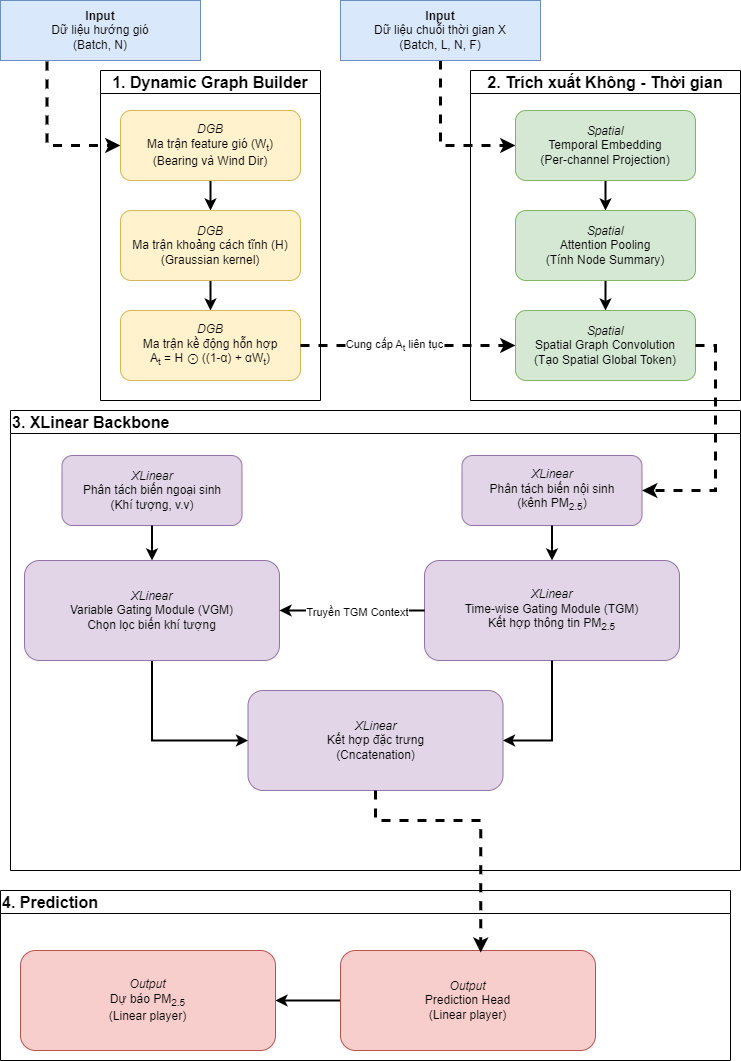
\includegraphics[scale=0.3]{image/Kiến trúc tổng quan ST-XLinear.drawio.png} 
    \caption{Kiến trúc tổng quan của mô hình đề xuất ST-XLinear}
    \label{fig:tongquanST-XLinear}
\end{figure}

ST-XLinear (Spatio-Temporal XLinear) là mô hình mạng thần kinh nhân tạo do đồ án đề xuất, kết hợp sức mạnh phân tích thời gian của kiến trúc XLinear \cite{Chen_2026} với cơ chế học biểu diễn không gian thông qua module Dynamic Graph Builder. Kiến trúc này được thiết kế nhằm khắc phục hai hạn chế lớn trong các nghiên cứu trước đây: (i) XLinear nguyên bản chỉ trích xuất đặc trưng theo chiều thời gian mà bỏ qua sự tương tác không gian giữa các trạm quan trắc, và (ii) các mô hình như E-STGCN \cite{panja2025estgcn} chỉ sử dụng ma trận kề tĩnh dựa trên khoảng cách, không phản ánh được tính động lực học của quá trình lan truyền ô nhiễm theo chiều gió.

Dựa trên Hình \ref{fig:tongquanST-XLinear}, luồng hoạt động của mô hình ST-XLinear được chia thành các giai đoạn chính như sau:

\paragraph{1. Xây dựng Ma trận kề động (Dynamic Graph Builder):} 
Thay vì sử dụng đồ thị cố định, module này liên tục tính toán ma trận kề $\mathbf{A}_t$ thay đổi theo thời gian thực dựa trên sự pha trộn giữa hai yếu tố:
\begin{itemize}
    \item \textit{Yếu tố bề mặt tĩnh (Khoảng cách)} $\mathbf{H}$: Khoảng cách vật lý (Haversine) giữa mọi cặp trạm $i$ và $j$ được chuyển hóa qua hàm Gaussian kernel: $H_{ij} = \exp(-d_{ij}^2/\sigma^2)$, thiết lập một nền tảng liên kết cơ sở cho các trạm gần nhau.
    \item \textit{Yếu tố động lực học (Gió)} $\mathbf{W}_t$: Tại mỗi bước thời gian $t$, góc phương vị (Bearing) $\beta_{ij}$ từ trạm $i$ đến $j$ được đối chiếu với hướng gió quan trắc $\theta_i^{(t)}$. Hệ số vận chuyển ô nhiễm được tính bằng $W_{ij}^{(t)} = \frac{\cos(\beta_{ij} - \theta_i^{(t)}) + 1}{2}$. Giá trị này đạt cực đại khi gió thổi thẳng từ trạm $i$ sang $j$.
    \item \textit{Tổng hợp:} Ma trận kề động cuối cùng bám sát nguyên lý vật lý môi trường được pha trộn qua công thức:
    \begin{equation}
        \mathbf{A}_t = \mathbf{H} \odot \left[(1 - \alpha) + \alpha \cdot \mathbf{W}_t\right]
    \end{equation}
\end{itemize}

\paragraph{2. Trích xuất đặc trưng không--thời gian:}
Dữ liệu đầu vào $\mathbf{X}$ (gồm biến mục tiêu $PM_{2.5}$ và các biến khí tượng) đi qua lớp \textbf{Temporal Embedding} (phép chiếu tuyến tính độc lập cho từng kênh) để chuyển thông tin thời gian thành vector đặc trưng. Sau đó, lớp \textbf{Attention Pooling} tổng hợp các kênh thành một Node Summary cho mỗi trạm.

Node Summary kết hợp cùng ma trận kề động $\mathbf{A}_t$ đi vào lớp tích chập không gian \textbf{Spatial GCN} để tổng hợp thông tin từ các trạm lân cận:
\begin{equation}
    \mathbf{S}^{\text{spatial}} = \text{LayerNorm}\left(\text{GELU}\left(\text{Linear}\left([\mathbf{S} \;\|\; \mathbf{A}_t \cdot \mathbf{S}]\right) + \mathbf{S}\right)\right)
\end{equation}
Kết quả sinh ra một \textit{Spatial Global Token} chứa đựng cả lịch sử thời gian cục bộ lẫn ngữ cảnh không gian toàn cục.

\paragraph{3. Khối xương sống XLinear (Backbone):}
Khác với XLinear nguyên bản sử dụng Learnable Token ngẫu nhiên, ST-XLinear tích hợp trực tiếp \textit{Spatial Global Token} vào luồng xử lý biến nội sinh. 
\begin{itemize}
    \item Khối \textbf{Time-wise Gating Module (TGM)} tiếp nhận biến nội sinh ($PM_{2.5}$) và ngữ cảnh không gian này để đánh giá tầm quan trọng của các mốc thời gian trong quá khứ.
    \item Ngữ cảnh đầu ra của TGM tiếp tục làm thông tin dẫn đường (guide context) đi vào khối \textbf{Variable-wise Gating Module (VGM)} để tiến hành sàng lọc nhiễu, quyết định biến ngoại sinh (nhiệt độ, độ ẩm, v.v.) nào có ý nghĩa lớn nhất đối với dự báo.
\end{itemize}
Hai đầu ra cuối cùng được Concatenation và đi qua lớp \textbf{Prediction Head} để xuất kết quả dự báo nồng độ $PM_{2.5}$ tại từng trạm.

Dưới đây là phần mô tả siêu tham số của mô hình, tập trung vào ý nghĩa và vai trò của từng siêu tham số:

\paragraph{Không gian Siêu tham số (Hyperparameter Space):}

\begin{table}[H]
\centering
\caption{Siêu tham số khối cấu trúc đồ thị mạng nội tại của ST-XLinear}
\label{tab:stxlinear_structure}
\renewcommand{\arraystretch}{1.3}
\begin{tabular}{p{3.8cm} p{10.5cm}}
\toprule
\textbf{Siêu tham số} & \textbf{Ý nghĩa} \\
\midrule
$seq\_len$ & Số bước thời gian lịch sử làm đầu vào cho mô hình. \\
$pred\_len$ & Số bước thời gian tương lai cần dự báo tại mỗi trạm. \\
$d\_model$ & Kích thước Embedding Dimension cho biểu diễn đặc trưng ẩn của chuỗi thời gian. \\
$t\_ff$ & Số nơ-ron trong lớp Feed-Forward của khối Temporal Gating Module. \\
$c\_ff$ & Số nơ-ron trong lớp Feed-Forward của khối Variable-wise Gating Module. \\
$dropout$ & Tỷ lệ Dropout áp dụng trong mạng để hạn chế Overfitting. \\
$alpha\_graph$ & Trọng số $\alpha \in [0,1]$ cân bằng giữa ma trận kề tĩnh (khoảng cách Haversine) và ma trận kề động (hướng gió). \\
\bottomrule
\end{tabular}
\end{table}

\begin{table}[H]
\centering
\caption{Siêu tham số khối huấn luyện và hàm mất mát của ST-XLinear}
\label{tab:stxlinear_optim}
\renewcommand{\arraystretch}{1.3}
\begin{tabular}{p{3.8cm} p{10.5cm}}
\toprule
\textbf{Siêu tham số} & \textbf{Ý nghĩa} \\
\midrule
$learning\_rate$ & Tốc độ học khởi tạo của thuật toán tối ưu AdamW. \\
$weight\_decay$ & Hệ số chính quy hóa L2 (Weight Decay) nhằm hạn chế Overfitting. \\
$T\_max$ & Số epoch cho nửa chu kỳ của bộ lập lịch CosineAnnealingLR. \\
$eta\_min$ & Giá trị tốc độ học tối thiểu mà bộ lập lịch Cosine không được giảm vượt quá. \\
$mse\_w$ & Trọng số cân bằng giữa thành phần MSE và MAE trong hàm CombinedLoss. \\
$delta$ & Ngưỡng chuyển đổi của hàm HuberLoss: dùng MSE khi sai số $< \delta$, dùng MAE khi sai số $\geq \delta$. \\
$epochs$ & Số vòng lặp huấn luyện tối đa trên toàn bộ tập dữ liệu. \\
$batch\_size$ & Số lượng mẫu dữ liệu mỗi Mini-batch. \\
$patience$ & Số epoch liên tiếp không cải thiện trên tập Validation trước khi dừng huấn luyện sớm (Early Stopping). \\
\bottomrule
\end{tabular}
\end{table}

\subsubsection{Phương pháp Ensemble}

Phương pháp Ensemble Learning là một kỹ thuật mạnh mẽ nhằm nâng cao hiệu suất dự báo và tính ổn định của hệ thống thông qua việc kết hợp dự đoán từ nhiều mô hình thành phần khác nhau. Nguyên lý cốt lõi của Ensemble dựa trên thực tế là các Base Learners, do sự khác biệt về kiến trúc và cách trích xuất đặc trưng, thường mắc phải các loại sai số phân bố khác nhau. Việc kết hợp chúng giúp triệt tiêu Variance (phương sai), khắc phục điểm yếu cục bộ của từng mô hình và giảm thiểu rủi ro quá khớp.

Trong hệ thống dự báo này, phương pháp Ensemble được thiết kế để kết hợp trực tiếp đầu ra của hai kiến trúc tiêu biểu có đặc thù phân tích khác nhau: mô hình dựa trên MLP (như XLinear, chuyên biệt về nắm bắt tính chu kỳ và lọc nhiễu ngoại sinh) và mô hình dựa trên đồ thị (như ESTGCN, chuyên biệt về khai thác dòng chảy không gian). Quy tắc kết hợp được sử dụng là Weighted Average. Cụ thể, giá trị dự báo cuối cùng $\hat{y}$ được tính bằng chập tuyến tính giữa giá trị dự báo của hai mô hình thành phần:
\begin{equation}
    \hat{y} = \alpha \cdot \hat{y}_{XLinear} + (1-\alpha) \cdot \hat{y}_{ESTGCN}
\end{equation}
trong đó, $\hat{y}_{XLinear}$ và $\hat{y}_{ESTGCN}$ lần lượt là dự báo nồng độ $PM_{2.5}$ xuất ra từ hai mô hình, và $\alpha \in [0, 1]$ là trọng số kết hợp.

Với phương pháp luận này, $\alpha$ không phải là tham số có thể học được (learnable parameter) bằng Gradient Descent trong quá trình huấn luyện mô hình, mà được xem như một Hyperparameter. Để đảm bảo tính khách quan và đạt hiệu suất tối ưu, $\alpha$ được xác định thông qua \textbf{Grid Search} trên tập Validation. Phương pháp dò tìm này được kiểm soát bởi các tham số không gian cấu hình chuyên biệt như sau:
\begin{table}[H]
\centering
\caption{Siêu tham số cấu hình Grid Search của phương pháp Ensemble}
\label{tab:ensemble_params}
\renewcommand{\arraystretch}{1.3}
\begin{tabular}{p{3.8cm} p{10.5cm}}
\toprule
\textbf{Siêu tham số} & \textbf{Ý nghĩa} \\
\midrule
$alpha$ ($\alpha$) & Trọng số kết hợp trong khoảng $[0, 1]$, quyết định tỷ lệ đóng góp kết quả của bộ ST-XLinear so với E-STGCN. \\
$metric$ & Chỉ số đánh giá tiêu chuẩn (ở đây là MAE trung bình) dùng để chọn giá trị $\alpha$ tối ưu nhất trên tập Validation. \\
$step$ & Khoảng cách giữa các giá trị $\alpha$ liền kề trong chuỗi quét Grid Search, quyết định độ mịn của mảng tìm kiếm. \\
\bottomrule
\end{tabular}
\end{table}
Cách tiếp cận này tận dụng được điểm mạnh từ các mô hình thành phần mà không làm tăng đáng kể tài nguyên tính toán.

\subsection{Các chỉ số đánh giá hiệu suất}

Để đánh giá một cách toàn diện, khách quan độ chính xác và khả năng tổng quát hóa của các mô hình dự báo $PM_{2.5}$, bước Evaluation đóng vai trò tối quan trọng. Không có một chỉ số đơn lẻ nào phản ánh hoàn hảo mọi khía cạnh của sai số dự báo; do đó, thông lệ nghiên cứu khoa học khuyến nghị sử dụng kết hợp nhiều chỉ số thống kê khác nhau để có cái nhìn đa chiều \cite{chai2014rmse, armstrong1992mape}. Trong đồ án này, các mô hình được so sánh chéo dựa trên bốn chỉ số đo lường chính.

\subsubsection{Root Mean Square Error (RMSE)}

Root Mean Square Error (Sai số toàn phương trung bình căn) là một trong những chỉ số đánh giá độ phân tán định lượng phổ biến nhất trong các bài toán hồi quy và dự báo môi trường. Nó được định nghĩa là căn bậc hai của trung bình cộng bình phương các khoảng cách giữa giá trị dự báo và giá trị quan trắc thực tế, có cùng đơn vị với biến mục tiêu ($\mu g/m^3$):
\begin{equation}
    RMSE = \sqrt{\frac{1}{N} \sum_{i=1}^{N} \left( y_i - \hat{y}_i \right)^2}
\end{equation}
trong đó $y_i$ là giá trị nồng độ $PM_{2.5}$ thực tế ở quan trắc thứ $i$, $\hat{y}_i$ là giá trị dự báo tương ứng, và $N$ là tổng số cỡ mẫu đánh giá.

Đặc tính quan trọng nhất của RMSE đến từ thao tác bình phương sai số trước khi lấy trung bình. Điều này khiến RMSE \textbf{phạt nặng} các sai số lớn (Outlier). Trong bối cảnh dự báo chất lượng không khí, đặc tính này cực kỳ hữu ích: việc mô hình bỏ sót một sự kiện nồng độ $PM_{2.5}$ tăng vọt đột ngột sẽ lập tức phản ánh bằng mức RMSE tăng cao. Theo Chai và Draxler (2014), RMSE đáng tin cậy hơn các chỉ số tuyệt đối khi phân phối sai số dự đoán tiến gần phân phối chuẩn Gaussian, đồng thời RMSE thỏa mãn bất đẳng thức tam giác để được xem là một Distance Metric hợp lệ \cite{chai2014rmse}.

\subsubsection{Mean Absolute Error (MAE)}

Mean Absolute Error (Sai số tuyệt đối trung bình) là một chỉ số đo lường độ lớn trung bình của sai số trong tập dự báo, bỏ qua dấu của chúng. Khác với RMSE, MAE không sử dụng thao tác bình phương mà trực tiếp lấy giá trị tuyệt đối của hiệu số giữa kết quả dự báo và quan trắc thực tế, sau đó tính trung bình cộng:
\begin{equation}
    MAE = \frac{1}{N} \sum_{i=1}^{N} \left| y_i - \hat{y}_i \right|
\end{equation}

Với cấu trúc tuyến tính này, mỗi sai số đóng góp vào giá trị trung bình với tỷ lệ thuận theo độ lớn tuyệt đối của riêng nó. Willmott và Matsuura (2005) lập luận rằng MAE là chỉ số tự nhiên và rõ ràng hơn so với RMSE \cite{willmott2005mae}. Do không phạt nặng các điểm ngoại lai, MAE mang tính Robust hơn trong các bộ dữ liệu có nhiều nhiễu bất thường, giúp đánh giá trung lực hiệu suất trung bình của mô hình. Độ chênh lệch giữa RMSE và MAE (RMSE $\geq$ MAE) phản ánh mức độ phân tán của phân phối sai số.

\subsubsection{Coefficient of Determination ($R^2$)}

Coefficient of Determination (Hệ số quyết định), thường được ký hiệu là $R^2$, là một chỉ số thống kê phản ánh tỷ lệ phần trăm sự biến thiên (phương sai) của biến mục tiêu mà mô hình dự báo có thể nắm bắt và giải thích được bằng các biến độc lập. Định nghĩa tổng quát của hệ số $R^2$ áp dụng cho cả hồi quy tuyến tính và phi tuyến tính (như mạng nơ-ron hay cây quyết định xgboost) \cite{nagelkerke1991r2, tirink2025aqi} được biểu diễn qua tỷ số giữa tổng bình phương phần dư ($SS_{res}$) và tổng bình phương toàn phần ($SS_{tot}$):
\begin{equation}
    R^2 = 1 - \frac{SS_{res}}{SS_{tot}} = 1 - \frac{\sum_{i=1}^{N} (y_i - \hat{y}_i)^2}{\sum_{i=1}^{N} (y_i - \bar{y})^2}
\end{equation}
trong đó, $\bar{y}$ là giá trị trung bình lượng $PM_{2.5}$ của dữ liệu thực tế đánh giá ($y_i$). 

Hệ số $R^2$ thường nhận giá trị trong khoảng $[0, 1]$. Giá trị $R^2$ tiến gần $1$ cho thấy mô hình bám sát gần như hoàn hảo mọi dao động của dữ liệu mục tiêu. Nếu $R^2 = 0$, mô hình chỉ dự đoán bằng giá trị trung bình $\bar{y}$, không học được quy luật nào. $R^2$ có thể âm khi mô hình dự báo kém hơn cả việc dùng giá trị trung bình.

\subsubsection{Mean Absolute Percentage Error (MAPE)}

Mean Absolute Percentage Error (Sai số phần trăm tuyệt đối trung bình) đo lường độ chính xác dưới dạng tỷ lệ phần trăm, mang lại ưu điểm vượt trội về khả năng diễn giải trực quan cho người trực tiếp sử dụng hệ thống so với các chỉ số số tuyệt đối (metric đơn vị) như RMSE hay MAE. Công thức MAPE là bình quân của sai số tuyệt đối quy đổi về tỷ lệ phần trăm dựa trên giá trị gốc:
\begin{equation}
    MAPE = \frac{100}{N} \sum_{i=1}^{N} \left| \frac{y_i - \hat{y}_i}{y_i} \right|
\end{equation}

Mặc dù phổ biến và dễ sử dụng để so sánh hiệu năng giữa các bộ dữ liệu khác nhau \cite{armstrong1992mape}, MAPE vẫn có một số nhược điểm đã được Armstrong và Collopy (1992) lưu ý. \textit{Thứ nhất}, khi giá trị thực tế ($y_i$) rất nhỏ hoặc bằng không, mẫu số sẽ khiến chỉ số tiến về vô cực. \textit{Thứ hai}, MAPE có thiên hướng phạt nặng Overpredict mạnh hơn Underpredict trên cùng độ lớn sai số tuyệt đối. Chính vì vậy, trong đồ án, MAPE được sử dụng đồng thời cùng MAE và RMSE để có cái nhìn tham chiếu đầy đủ.
\subsection{Các phương pháp chuẩn hóa dữ liệu}

Trong các bài toán dự báo chuỗi thời gian đa biến, đặc biệt là dự báo nồng độ chất ô nhiễm như $PM_{2.5}$, các biến đầu vào (khí tượng, nồng độ các chất) thường có thang đo, đơn vị và đặc tính phân phối rất khác biệt. Việc đưa trực tiếp các giá trị thô này vào các mạng nơ-ron học sâu hoặc các thuật toán tối ưu hóa bằng gradient có thể dẫn đến hiện tượng bùng nổ đạo hàm, hội tụ chậm, hoặc khiến mô hình bị thiên lệch về phía các đặc trưng có giá trị tuyệt đối lớn. 

Do đó, việc tiền xử lý và chuẩn hóa dữ liệu là bước bắt buộc. Dựa trên quá trình phân tích đặc thù phân phối của từng nhóm biến quan trắc \cite{tukey1977eda}, hệ thống áp dụng linh hoạt các phương pháp biến đổi và chuẩn hóa được hỗ trợ thông qua thư viện Scikit-learn \cite{pedregosa2011sklearn} như sau:

\subsubsection{Biến đổi Logarit (Log1p)}
Biến đổi logarit được áp dụng chủ yếu cho các biến có phân phối lệch phải với độ lệch lớn, một hiện tượng rất phổ biến ở các đo lường nồng độ chất ô nhiễm cục bộ. Nhằm xử lý an toàn các trường hợp giá trị bằng không (như lượng mưa hoặc nồng độ cực thấp), hệ thống sử dụng hàm $\log1p$ thay vì logarit tự nhiên tiêu chuẩn \cite{box1964analysis}:
$$x' = \ln(1 + x)$$
Phép biến đổi phi tuyến này giúp thu hẹp đuôi phân phối dài, kéo cấu trúc dữ liệu về dạng gần đối xứng hơn. Điều này làm giảm đáng kể mức độ ảnh hưởng của các giá trị cực đoan trước khi dữ liệu được đưa qua các bộ chuẩn hóa tuyến tính.

\subsubsection{Cắt xén ngoại lai (Clipping Percentile)}
Đối với các biến chứa giá trị ngoại lai dị thường sinh ra do lỗi cảm biến hoặc các hiện tượng thời tiết cực đoan đột ngột, việc giữ nguyên chúng có thể làm hẹp phương sai của dải giá trị bình thường sau khi chuẩn hóa. Kỹ thuật cắt xén, dựa trên nền tảng của phương pháp Winsorization \cite{hastings1947low}, được hệ thống áp dụng ở các ngưỡng phân vị cao (ví dụ: percentile thứ 99 hoặc 99,5):
$$x' = \min(x, P_q)$$
trong đó $P_q$ là giá trị tại phân vị thứ $q$ của tập dữ liệu. Phương pháp này thiết lập một ngưỡng trần an toàn, gọt bớt các đỉnh nhọn dị biệt mà không làm biến dạng cấu trúc phân phối của phần lớn dữ liệu hợp lệ còn lại.

\subsubsection{Chuẩn hóa Z-score (StandardScaler)}
Phương pháp Standard Scaler chuẩn hóa dữ liệu dựa trên nguyên lý dịch chuyển và thay đổi tỷ lệ, giả định biến có phân phối xấp xỉ phân phối chuẩn. Mỗi điểm dữ liệu được chuyển đổi thành điểm Z-score thông qua việc trừ đi giá trị trung bình ($\mu$) và chia cho độ lệch chuẩn ($\sigma$) của toàn tập mẫu \cite{han2011data, lecun1998efficient}:
$$x' = \frac{x - \mu}{\sigma}$$
Sau khi chuẩn hóa, biến đầu ra sẽ có trung bình bằng $0$ và phương sai bằng $1$. Kỹ thuật này được áp dụng cho các đặc trưng khí tượng có phân phối gần chuẩn và ít chứa điểm ngoại lai, điển hình như nhiệt độ, nhiệt độ điểm sương, độ ổn định nhiệt hoặc nhiệt độ đất.

\subsubsection{Chuẩn hóa mạnh (RobustScaler)}
Với các biến có phân phối không chuẩn và chứa đựng nhiều điểm ngoại lai thực tế — ví dụ như nồng độ $SO_2$, $O_3$, tốc độ gió hoặc chính bản thân biến mục tiêu $PM_{2.5}$ — các chỉ số $\mu$ và $\sigma$ ở phương pháp chuẩn sẽ bị kéo lệch nghiêm trọng. Robust Scaler khắc phục điểm yếu này bằng cách sử dụng các đại lượng thống kê kháng nhiễu là Median ($Q_2$) và Interquartile Range ($IQR = Q_3 - Q_1$) \cite{rousseeuw1993robust}:
$$x' = \frac{x - Q_2}{Q_3 - Q_1}$$
Bằng cách loại bỏ sự chi phối của các giá trị cực đoan tại hai đầu mút phân phối, Robust Scaler giúp mô hình học sâu nắm bắt được tri thức cốt lõi của chuỗi thời gian mà không bị "đánh lừa" bởi các đợt nhiễu sóng ngắn hạn.

\subsubsection{Chuẩn hóa Min-Max (MinMaxScaler)}
Phương pháp Min-Max thực hiện phép co giãn tuyến tính toàn bộ dải dữ liệu về một khoảng giới hạn cố định (thường là $[0, 1]$) \cite{han2011data}:
$$x' = \frac{x - x_{min}}{x_{max} - x_{min}}$$
Kỹ thuật này đặc biệt tối ưu cho các biến mà bản chất vật lý của chúng đã có biên độ và giới hạn cực trị rõ ràng, chẳng hạn như độ ẩm tương đối ($0 - 100\%$), độ che phủ mây, độ ẩm đất, hoặc các biến lượng mưa đã qua cắt xén.

\subsection{Các công trình nghiên cứu liên quan}

Để xây dựng cơ sở khoa học và định vị được những đóng góp của đồ án, việc rà soát và đánh giá các nghiên cứu đi trước về dự báo nồng độ ô nhiễm $PM_{2.5}$ cả trong nước và quốc tế là hết sức cần thiết. Các hướng tiếp cận đang phân hóa rất đa dạng dựa trên cả mô hình vật lý--hóa học truyền thống và các phương pháp Machine Learning / Deep Learning hiện đại.

\subsubsection{Nghiên cứu trong nước}

Tại Việt Nam, các nghiên cứu chuyên sâu về phân bố ô nhiễm không khí và ảnh hưởng sức khỏe đang ngày càng được chú trọng do mức độ báo động tại các đô thị lớn. Khởi điểm từ khía cạnh vĩ mô, nghiên cứu của Bui và Nghiem (2025) đã chứng minh được mối liên hệ tuyến tính giữa mật độ đô thị hóa và mức độ ô nhiễm thông qua mô phỏng hồi quy trên 63 tỉnh thành: mỗi 1\% gia tăng đô thị hóa sẽ kéo theo nồng độ $PM_{2.5}$ tăng \textbf{0,54 $\mu g/m^3$} \cite{bui2025urbanization}. Cùng đánh giá trên bài toán y tế công cộng, Le et al. (2024) \cite{le2024environmental} và Hoang et al. (2023) \cite{hoang2023health} đã định lượng được mối liên hệ giữa phơi nhiễm bụi mịn thứ cấp với các bệnh lý tim mạch và hô hấp, đồng thời ước tính thiệt hại kinh tế lên đến hàng trăm triệu USD mỗi năm --- cho thấy tiềm năng phòng tránh hàng nghìn ca tử vong sớm nếu duy trì được chất lượng không khí ở mức thời kỳ giãn cách COVID-19. 

Về phương pháp mô hình hóa, các nghiên cứu trong nước chủ yếu sử dụng hệ thống mô phỏng vật lý--hóa học truyền thống, tiêu biểu là CMAQ (Community Multiscale Air Quality). 
Cụ thể, Ho et al. (2025) sử dụng mô hình này kết hợp với hồ sơ phát thải giao thông nhằm phân tích cơ chế lan truyền các chất ô nhiễm tại Hà Nội theo biến động mùa vụ \cite{ho2025assessment}. Tương tự, Nguyen et al. (2024) triển khai mô phỏng trên hệ thống CMAQ kết hợp WRF, đạt khả năng bao phủ không gian rộng nhưng sai số vẫn ở mức cao ($MAPE \approx 63\%$) trong các điều kiện khí tượng phức tạp \cite{nguyen2024cmaq}. 
Bên cạnh đó, Dam et al. (2024) thông qua phân tích dữ liệu quan trắc thực địa đã chỉ ra gradient nồng độ $PM_{2.5}$ theo chiều thẳng đứng rất rõ rệt, liên quan chặt chẽ đến hiện tượng nghịch nhiệt: nồng độ ở 30m là 50--84 $\mu g/m^3$, trong khi ở 320m chỉ còn 34--40 $\mu g/m^3$ \cite{dam2024pm25}. 

\subsubsection{Nghiên cứu ngoài nước}

Trái ngược với sự thống trị của các mô hình cơ học hóa tại Việt Nam, xu thế nghiên cứu toàn cầu trong vài năm trở lại đây tập trung cao độ vào nhóm Machine Learning và Deep Learning.

\textbf{Ứng dụng Gradient Boosting:} XGBoost và LightGBM thường được triển khai nhờ tốc độ xử lý nhanh, minh bạch dữ liệu đầu vào. Tırınk (2025) đã so sánh hiệu năng dự báo AQI trên bộ dữ liệu 8 năm tại Türkiye và kết luận XGBoost đạt hiệu năng vượt trội so với LightGBM và SVM \cite{tirink2025aqi}. Với yêu cầu IoT ở trạm giám sát rẻ tiền biên, Al-Nuaimi et al. (2025) đã nén mô hình XGBoost xuống chỉ 13 kB mà vẫn duy trì hiệu năng chấp nhận được \cite{alnuaimi2025lightweight}.

\textbf{Ứng dụng mô hình Deep Learning Temporal:} Các mô hình hồi quy LSTM và GRU khai thác phụ thuộc thời gian thông qua cơ chế cổng. Silveira et al. (2025) cho thấy LSTM đạt hiệu suất cao trên cả bài toán Single-step lẫn Multi-horizon nhờ khả năng giải quyết vấn đề Vanishing Gradient \cite{silveira2025lstmgru}. Zhang et al. (2025) \cite{zhang2025cnnlstm} đề xuất kết hợp CNN và LSTM để trích xuất đặc trưng cục bộ cho dự báo $PM_{2.5}$ tại Bắc Kinh (đạt $RMSE = 5{,}236$ trong biến thiên 6 giờ). Gần đây, He et al. (2024) kết hợp BiLSTM và GRU để nắm bắt phụ thuộc thời gian cả hai chiều \cite{he2024bilstmgru}. Tuy vậy, hạn chế chung của họ RNN vẫn là xử lý tuần tự, không thể song song hóa, dẫn đến thời gian huấn luyện lớn trên chuỗi dài.

\textbf{Kiến trúc Transformer và mô hình Spatio-Temporal:} Để khắc phục hạn chế về tính tuần tự, các kiến trúc Transformer đã được áp dụng vào dự báo chuỗi thời gian. Điển hình, iTransformer \cite{liu2024itransformer} đảo ngược chiều Self-Attention từ chiều thời gian sang chiều biến, cho phép xử lý song song hiệu quả. Về mô hình không--thời gian, Panja et al. (2025) đề xuất E-STGCN kết hợp Graph Convolution với LSTM: ma trận kề được xây dựng từ Gaussian kernel trên khoảng cách Haversine giữa các trạm, cho phép mô hình nắm bắt sự lan truyền $PM_{2.5}$ theo cấu trúc không gian \cite{panja2025estgcn}. 

\subsubsection{Nhận xét và khoảng trống nghiên cứu}

Việc tổng hợp các tài liệu của học giả trong nước lẫn quốc tế trên nhiều phương diện (sức khỏe cộng đồng \cite{hoang2023health}, hóa môi trường \cite{ho2025assessment}, mạng học sâu nâng cao \cite{liu2024itransformer}) cho thấy bức tranh tổng quan đồng thời làm lộ rõ một số khoảng trống tồn đọng trong nền tảng nghiên cứu ứng dụng cho bài toán tại Việt Nam:

\begin{enumerate}
    \item \textbf{Thiếu hụt hệ thống đánh giá đối chuẩn (Benchmark) đồng thời:} Trên cùng dữ liệu quan trắc $PM_{2.5}$ tại nước ta, đa số các công trình hoặc dùng các bộ quan sát quá cũ (thập kỷ trước) để thử thuật toán Machine Learning nhỏ lẻ, hoặc dùng khung mô phỏng truyền thống tốn kém máy chủ CMAQ. Chưa có nghiên cứu nào xây dựng hệ thống Benchmark so sánh trực tiếp giữa Machine Learning cổ điển, Sequence Model, Transformer và Spatio-Temporal Graph trên bộ dữ liệu Việt Nam nhiều năm với khung đánh giá Multi-horizon.
    
    \item \textbf{Cấu trúc không gian đồ thị chưa khai thác đặc tính động lực học lưu chất:} Hầu hết các kỹ thuật Graph Network truyền thống trong dự báo dòng chảy ô nhiễm không khí (kể cả E-STGCN mới nhất) đều áp dụng mô hình liên kết ma trận đồ thị dạng lưới bằng khoảng cách tĩnh \cite{panja2025estgcn}. Cách tiếp cận này bỏ qua vai trò quyết định của gió trong quá trình vận chuyển ô nhiễm: một trạm nằm xuôi theo chiều gió có khả năng ảnh hưởng cao hơn rất nhiều so với trạm ngược gió, ngay cả khi khoảng cách vật lý nhỏ hơn.
    
    \item \textbf{Quá trình Feature Engineering chưa dựa trên nguyên lý khí quyển học:} Điển hình do giới hạn về mặt dữ liệu, công tác thiết kế đặc trưng bổ trợ thường được bỏ qua đối với vùng nhiệt đới phức tạp tự nhiên. Chưa có thực nghiệm nào bóc tách trích xuất các dạng chỉ báo liên quan đến aerosol sulfate hay chỉ số quy luật bức xạ của ánh sáng làm Context Guide cho các kênh DL model Việt Nam.
\end{enumerate}

Những khoảng trống nêu trên chính là cơ sở để đồ án đề xuất hệ thống ST-XLinear tích hợp Dynamic Graph Builder cùng quy trình Feature Engineering dựa trên nguyên lý khí quyển học, được trình bày chi tiết tại các chương tiếp theo.

